\documentclass[tikz,border=10pt]{standalone}
\usepackage{tikz}
\begin{document}
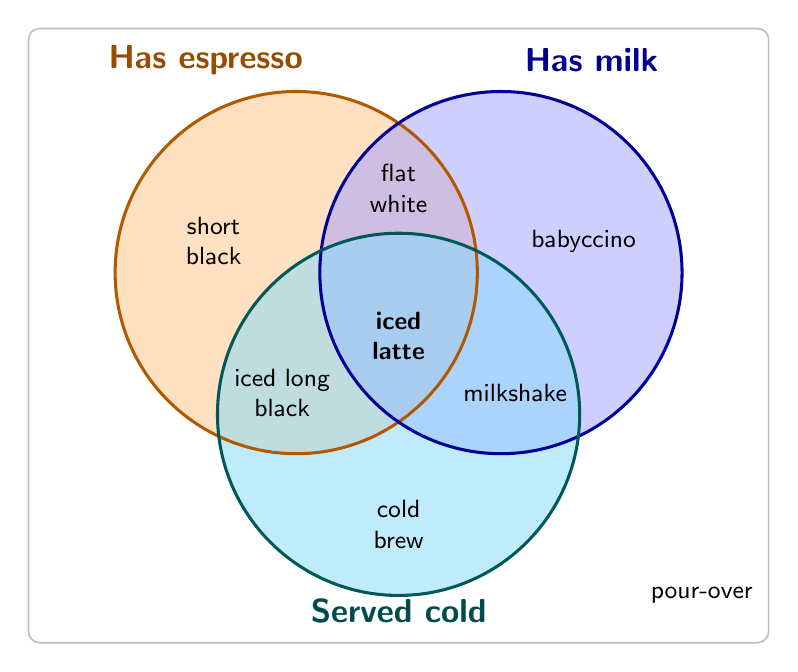
\begin{tikzpicture}[font=\sffamily, line join=round]
  % Universe (outside region)
  \draw[gray!50, line width=0.6pt, rounded corners=4pt] (-4.7,-3.95) rectangle (4.7,3.85);

  \def\R{2.3}
  \coordinate (E) at (-1.3,0.75);
  \coordinate (M) at ( 1.3,0.75);
  \coordinate (C) at ( 0,-1.05);

  % Filled circles with transparency so overlaps are visible
  \begin{scope}[blend group=normal]
    \fill[orange!45, fill opacity=0.55] (E) circle (\R);
    \fill[blue!35,   fill opacity=0.55] (M) circle (\R);
    \fill[cyan!45,   fill opacity=0.55] (C) circle (\R);
  \end{scope}

  % Circle outlines
  \draw[line width=1.1pt, orange!70!black] (E) circle (\R);
  \draw[line width=1.1pt, blue!60!black]   (M) circle (\R);
  \draw[line width=1.1pt, teal!70!black]   (C) circle (\R);

  % Circle labels, placed on the non-overlapping arcs
  \node[font=\sffamily\bfseries\large, orange!60!black] at (-2.45,3.45) {Has espresso};
  \node[font=\sffamily\bfseries\large, blue!55!black]   at ( 2.45,3.45) {Has milk};
  \node[font=\sffamily\bfseries\large, teal!60!black]   at ( 0,-3.55) {Served cold};

  % Drinks: one in each region
  \tikzset{drink/.style={align=center, font=\sffamily\small, text=black}}

  % Espresso only
  \node[drink] at (-2.35,1.15) {short\\black};
  % Milk only
  \node[drink] at (2.35,1.15) {babyccino};
  % Cold only
  \node[drink] at (0,-2.45) {cold\\brew};
  % Espresso + milk, not cold
  \node[drink] at (0,1.82) {flat\\white};
  % Espresso + cold, no milk
  \node[drink] at (-1.48,-0.78) {iced long\\black};
  % Milk + cold, no espresso
  \node[drink] at (1.48,-0.78) {milkshake};
  % All three
  \node[drink, font=\sffamily\small\bfseries] at (0,-0.05) {iced\\latte};
  % Outside all three
  \node[drink] at (3.85,-3.35) {pour-over};

\end{tikzpicture}
\end{document}
